\documentclass[11pt, oneside]{article} 
\usepackage{geometry}
\geometry{letterpaper} 
\usepackage{graphicx}
	
\usepackage{amssymb}
\usepackage{amsmath}
\usepackage{parskip}
\usepackage{color}
\usepackage{hyperref}

\graphicspath{{/Users/telliott_admin/Dropbox/Tex/png/}}
% \begin{center} 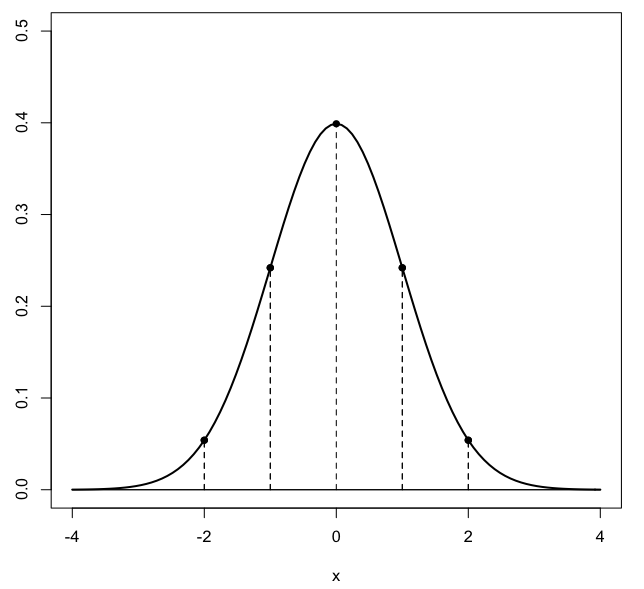
\includegraphics [scale=0.4] {gauss3.png} \end{center}

\title{Spivak's "hard" theorems}
\date{}

\begin{document}
\maketitle
\Large
Spivak's \emph{Calculus} lists three theorems that he calls "hard theorems" in Chapter 7  and then proves them in Chapter 8.  They are at the heart of the transition between the Archimedean principle, "completeness" and the idea of least upper bounds on the one hand, and the mean value theorem, on the other.

\subsection*{Bolzano's theorem}

$\bullet$  If $f$ is continuous on $[a,b]$ and $f(a) < 0 < f(b)$ then there is some $x$ in $[a,b]$ such that $f(x) = 0$.

\subsection*{f is bounded above}

$\bullet$  If $f$ is continuous on $[a,b]$ then $f$ is bounded above on $[a,b]$, that is, there is some number $N$ such that $f(x) \le N$ for all $x$ in $[a,b]$.

\subsection*{mini-max}

There is a maximum (and a minimum) value for $f$ on $[a,b]$

$\bullet$  If $f$ is continuous on $[a,b]$ then there is a number $y$ in $[a,b]$ such that $f(y) \ge f(x)$ for all $x$ in $[a,b]$.

\subsection*{proofs}
\begin{center} 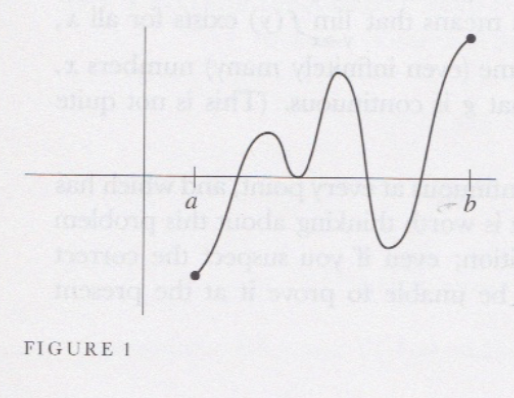
\includegraphics [scale=0.4] {spivak1.png} \end{center}

$\bullet$  If $f$ is continuous on $[a,b]$ and $f(a) < 0 < f(b)$ then there is some $x$ in $[a,b]$ such that $f(x) = 0$.

We proved this theorem in the write-up titled "bolzano".

$\bullet$  If $f$ is continuous on $[a,b]$ then $f$ is bounded above on $[a,b]$, that is, there is some number $N$ such that $f(x) \le N$ for all $x$ in $[a,b]$.

\begin{center} 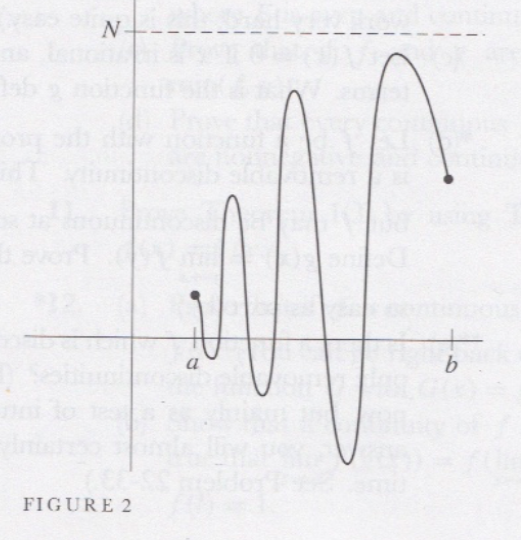
\includegraphics [scale=0.4] {spivak2.png} \end{center}



\newpage
\begin{center} 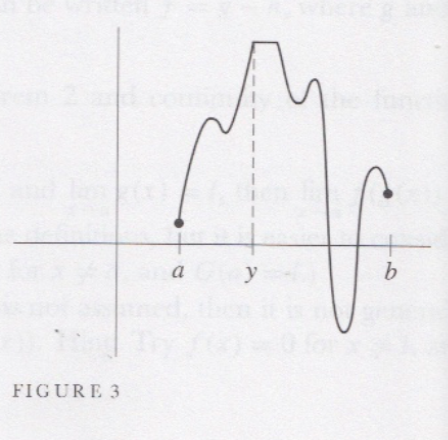
\includegraphics [scale=0.4] {spivak3.png} \end{center}

\end{document}}